\newpage
\chapter{Simulations}
\section{Introduction}

In the previous chapter, the theoretical framework for the various tracking filters and the adaptive techniques used for tracking our target of interest in the bistatic range and Doppler domain were explored. The primary objective of this dissertation is to implement these tracking filters and rigorously evaluate their performance through simulations. The simulations presented in this chapter are conducted using MATLAB code and \ac{FERS}.
\newline 
\newline
In section 4.1, the \ac{Radar} system overview is outlined. The setup of the simulation environment using \ac{FERS} is discussed in section 4.2, followed by a detailed discussion of the results from the \ac{Radar} processing chain simulations in section 4.3. The formulation of target dynamics is covered in section 4.4. Lastly, the implementation of the tracking filters and the \ac{MTT} are discussed in section 4.5. The evaluation metrics for assessing the performance of the tracking filters is addressed in the next chapter.

\subsection{Radar System Overview}

\ac{Radar} systems can be configured with various architectures, each optimized for specific objectives. In the simulations conducted within this section, the focus is on modelling the targets of interest within a \ac{Radar} environment. Following this, the \ac{Radar} processing chain and the \ac{MTT} system implementation is considered. The flow diagram in Figure \ref{fig:simulationRadar} depicts the key components involved in the overall \ac{Radar} simulation, including the \ac{MTT} system. From the \ac{Radar} System Overview, certain components, such as \ac{DPI} and clutter cancellation, fall outside of the primary scope of this research. However, validating the functionality of these components is crucial to ensure successful target tracking.
\newline
\begin{figure}[H]
    \centering
    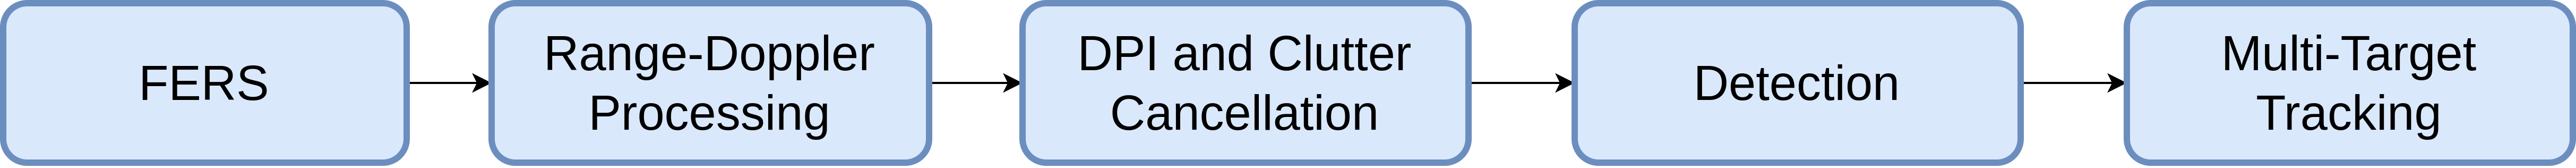
\includegraphics[width=0.95\linewidth]{Figure/radarOverview.drawio.png}
    \vspace{0.5em} 
    \caption{Flow diagram for  Radar System Overview for Simulations.}
    \label{fig:simulationRadar}
\end{figure}

 The simulations will focus on the implementation of some of the components. These components are detailed as follows:

\begin{itemize}

\item \textbf{\ac{FERS}\\} Simulates the behaviour of the \ac{Radar} system, defining various components within the \ac{Radar} environment. The discussion and usage of \ac{FERS} are covered in section 4.2.

\item \textbf{Range and Doppler Processing:}\\
This involves processing the  \ac{Radar} signals from \ac{FERS} into the bistatic range and Doppler domain.

\item \textbf{DPI and Clutter Cancellation:}\\
This component addresses the removal of \ac{DPI} and clutter from the bistatic range and Doppler map. Validation is performed to ensure the algorithm operates correctly.

\item \textbf{Detection:}\\
Detection of targets is achieved using a \ac{CA-CFAR} detection filter, followed by a clustering algorithm to determine target centroids.

\item \textbf{Multi-Target Tracking:}\\
This involves tracking multiple targets based on observations, which includes data association, track management and target state estimation using tracking filters.

\end{itemize}

\section{Flexible Extensible Radar Simulator}

\ac{FERS} was developed from a Ph.D. thesis presented in \cite{fersMarc}, which was based on creating a simulator that supports various \ac{Radar} system configurations. The simulator was introduced as an open-source project to address certain limitations of custom \ac{Radar} simulators, offering the capability to handle an arbitrary number of transmitter/receiver nodes and targets distributed across space and time \cite{inggs2009extensible}. Full documentation of the \ac{FERS} simulator can be found on the project's \href{https://github.com/stpaine/FERS/wiki}{GitHub Wiki page}.
\newline
\begin{figure}[H]
    \centering
    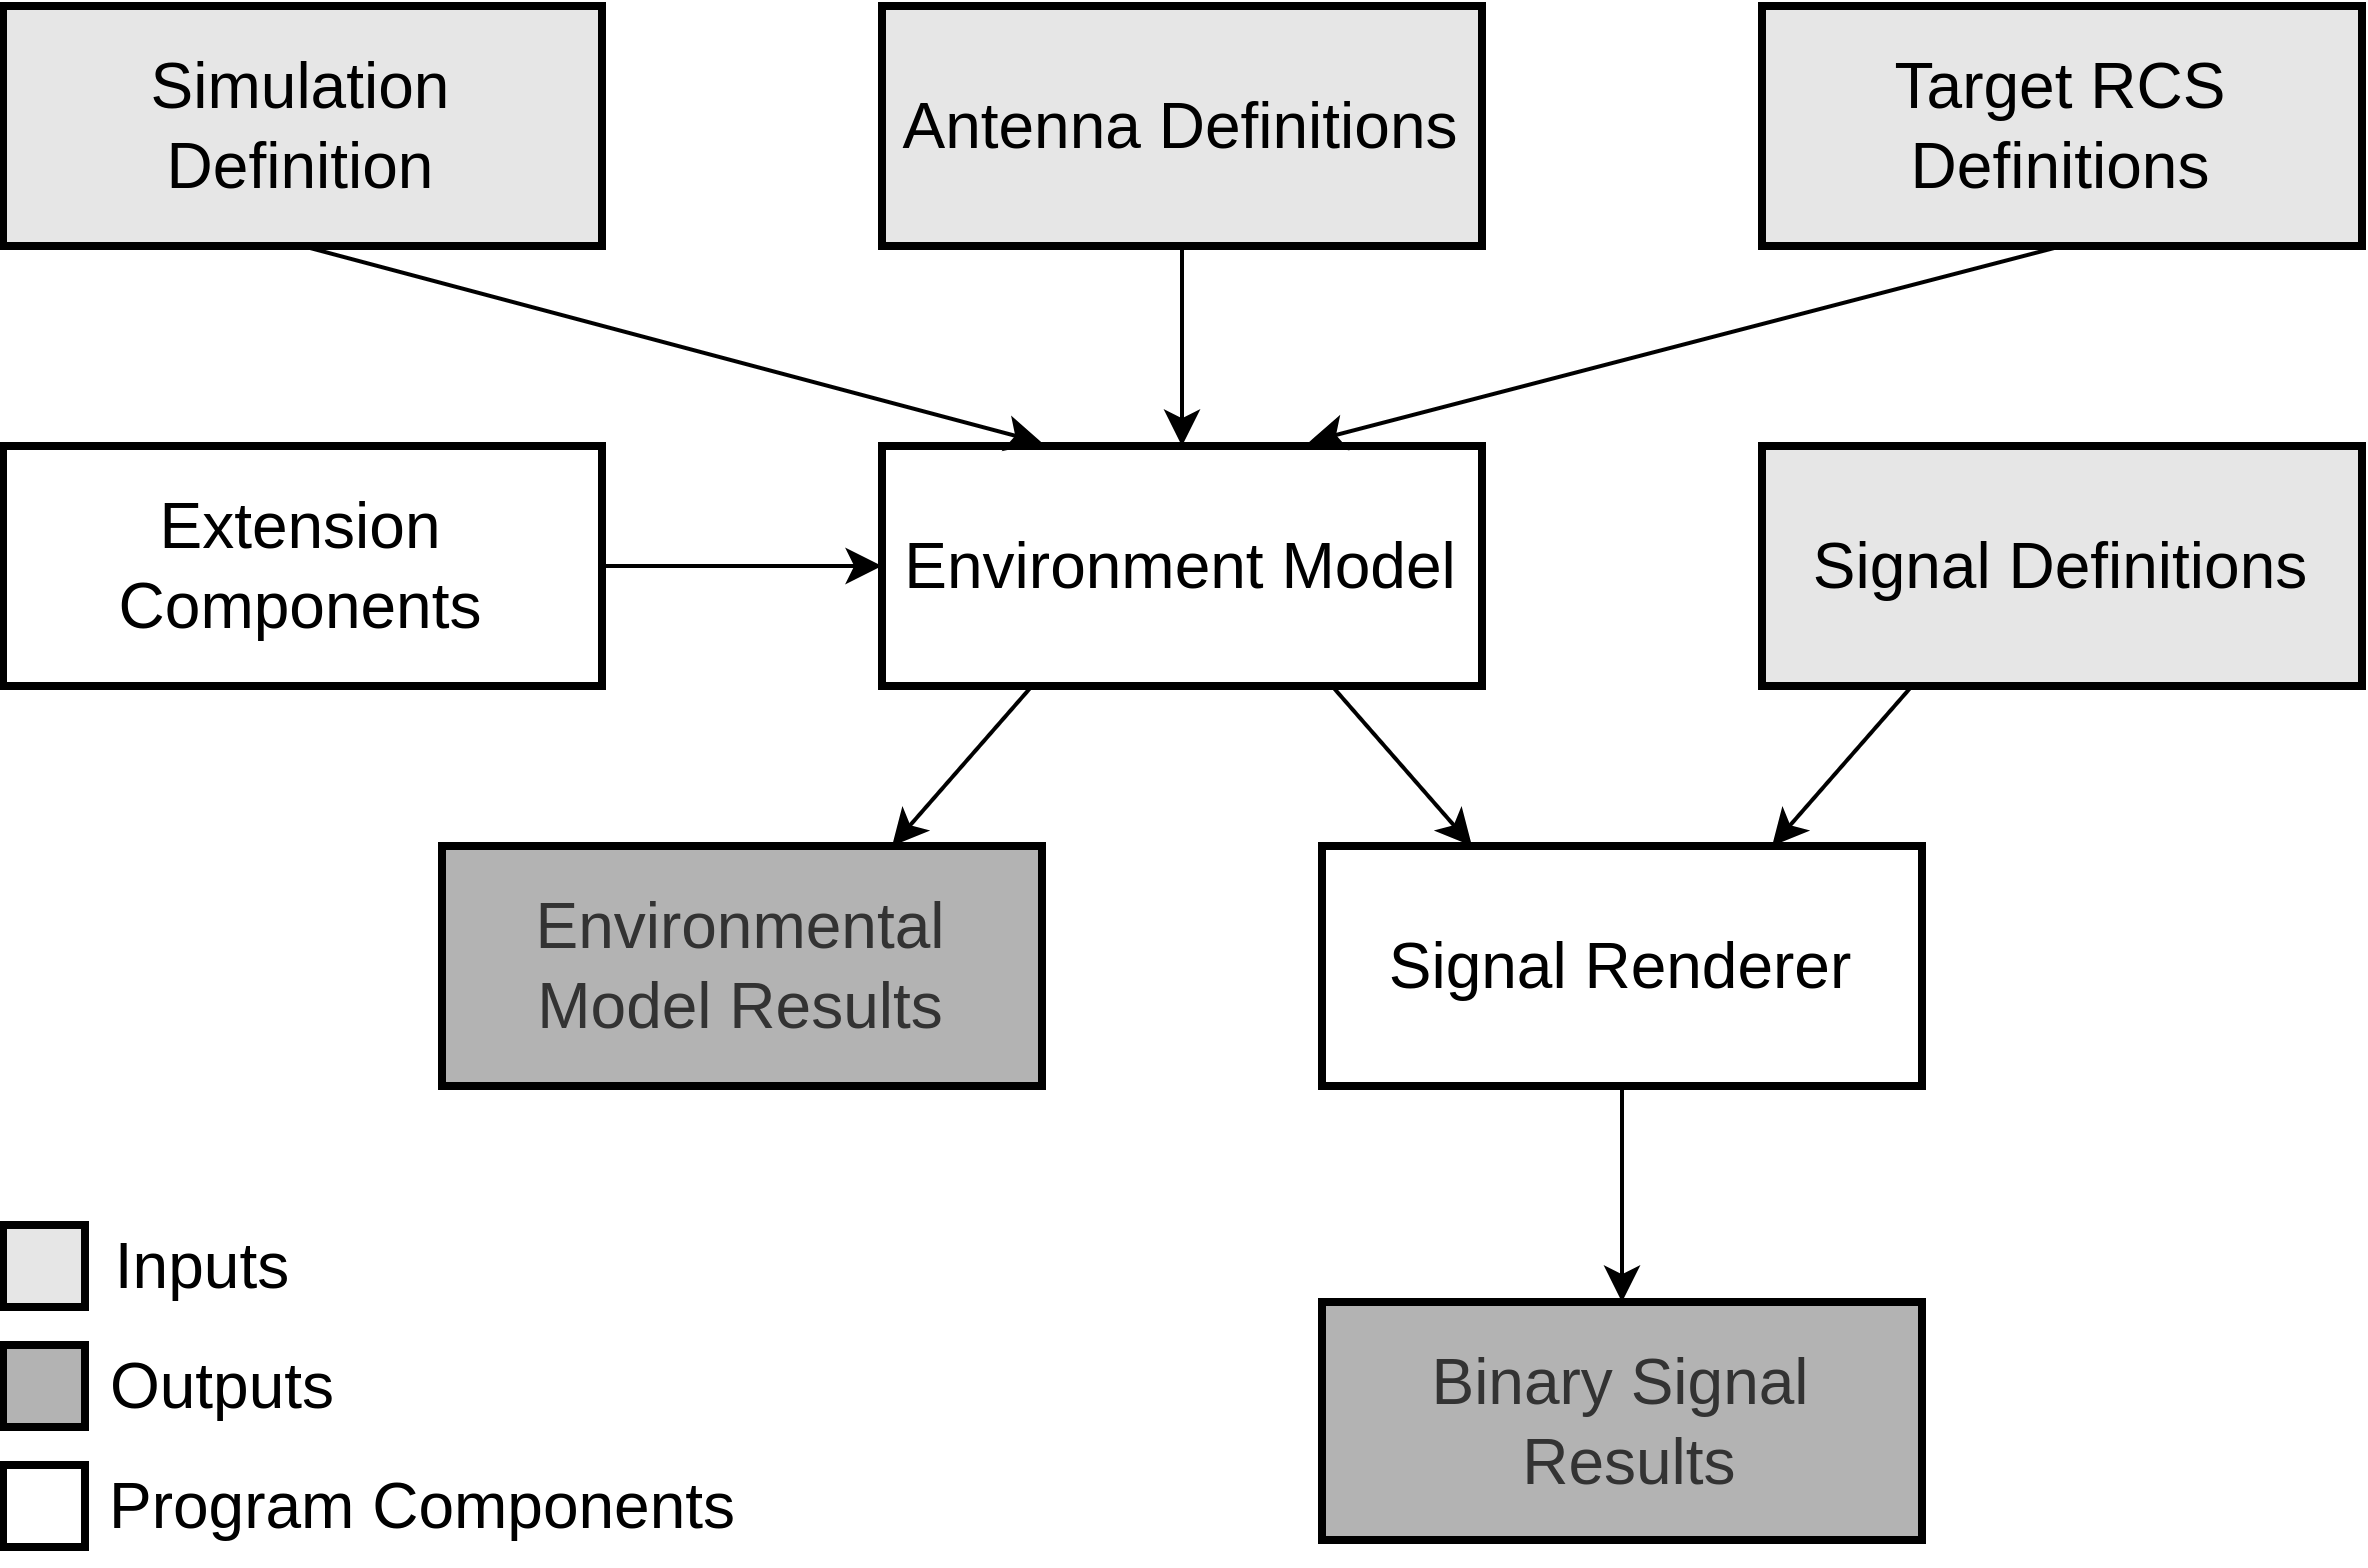
\includegraphics[width=0.75\linewidth]{Figure/fersDataflow.drawio (2).png}
    \vspace{2em}
    \caption{The FERS data flow diagram illustrates the various components  within the FERS Simulator.}
        \label{fig:fers-flow}
\end{figure}

\subsection{FERS Simulation Setup and Configuration}
\ac{FERS} simulator requires several key inputs to define the simulation environment as illustrated in Figure \ref{fig:fers-flow} from \cite{inggs2009extensible}. These inputs include the \ac{Radar} system configuration, environmental parameters, antenna characteristics, the transmitted waveform, and the target's \ac{RCS}. The simulator uses an \ac{XML} file as the input format.

The specific parameters used in \ac{FERS} to achieve the simulation objectives are discussed here. Firstly, the input definitions are discussed, followed by an explanation of the output data that constitutes our simulation results. The internal workings of the simulator are beyond the scope of this project; instead, the focus is on how the input parameters are utilized to produce results that will be validated against the theoretical expectations further in the simulations.


\subsection{Simulation Definition}
The simulation definition in \ac{FERS} consists of several details..

\subsubsection{FERS Simulation Parameters}

The main parameters used in \ac{FERS} for the bistatic \ac{Radar} setup are described in Table \ref{Sim_par_FERS}, the other configurations are outlined in the \ac{XML} code for the different scenarios.

\begin{table}[h]
\centering
\caption{Simulation Parameters.}
\label{Sim_par_FERS}
\begin{tabular}{ll}
\hline
\textbf{Parameter} & \textbf{Value} \\
\hline
Start Time & 0 \\
End Time & Duration of Simulation (s) \\
Sampling Rate & 200 kHz \\
\ac{ADC} Bits & 16 \\
Propagation Speed & Speed of Light (\textit{c}) \\
\hline
\end{tabular}
\end{table}

\subsubsection{Pulse}
Describes the transmitted waveform parameters, including power and carrier frequency. An \ac{FM} waveform signal recorded in Malmesbury is used as the transmitted waveform. The carrier frequency and power are also varied depending on the scenario being simulated.

\subsubsection{Timing}
Specifies the timing source parameters; the frequency of the clock is set to 200 kHz.

\subsubsection{Platform}
Details the platform, its position and its components, such as a receiver, transmitter or target. Three platforms for the transmitter, surveillance and direct receiver channels, along with additional platforms for the targets that are used.

\subsection{Antenna and Target Definition}
The Antenna parameter in the XML defines the antenna gain and pattern. The receiver antennas are set to use directional antennas with a 'sinc' function pattern. The target \ac{RCS} and trajectories are configured depending on the scenario being simulated.

\subsection{Binary Signal Results}
The output data from \ac{FERS} is stored as 64-bit floating point samples in an HDF5 binary file. This file contains the received signals from the receiver terminals as baseband signals (quadrature and in-phase components). These signals are used for processing in the subsequent section to resolve the range and Doppler map.


\section{Processing Chain Implementation}
The components of the processing chain are all implemented in MATLAB code. In the first subsection, the results from the range and Doppler processing using the results from \ac{FERS} are discussed.

\subsection{Range and Doppler Processing}
The problem of target localization using cross-correlation is discussed in Chapter 2 with Equation (\ref{crossamb})  using the ambiguity function. From the signals extracted from the \ac{FERS} output files, the individual signals are reconstructed into complex signals for both the reference and surveillance channel signals. The processing of the signals to compute the \ac{ARD} map  can be written in discrete time as: 

\begin{equation}
    \left| \Psi(\tau, v) \right| = \left| \sum_{n=0}^{N-1} s_E(n) s_R^*(n-\tau) e^{j 2\pi v n/N} \right|
\end{equation}

where \( \Psi(\tau, v)\) is the Amplitude/Range/Doppler map, \(s_E(n)\) represents the echo signal, and \(s_R^*(n-\tau)\) is the complex conjugate of the reference signal extracted from the surveillance channel. To illustrate a simple case of target detection using the received signals from \ac{FERS}, a bistatic \ac{Radar} setup is configured with two receivers (surveillance and reference), a single transmitter and a single target as observed in Figure \ref{fig:ferssetup}. The transmitter is modelled as an \ac{FM} band omni-directional illuminator in \ac{FERS}, using an isotropic antenna that transmits an \ac{FM} waveform with a centre frequency of 94 MHz. The receivers are modelled as directional antennas and the baseline separation between the receivers and the transmitter is 12.5 km.
\newline
\begin{figure}[H]
    \centering
    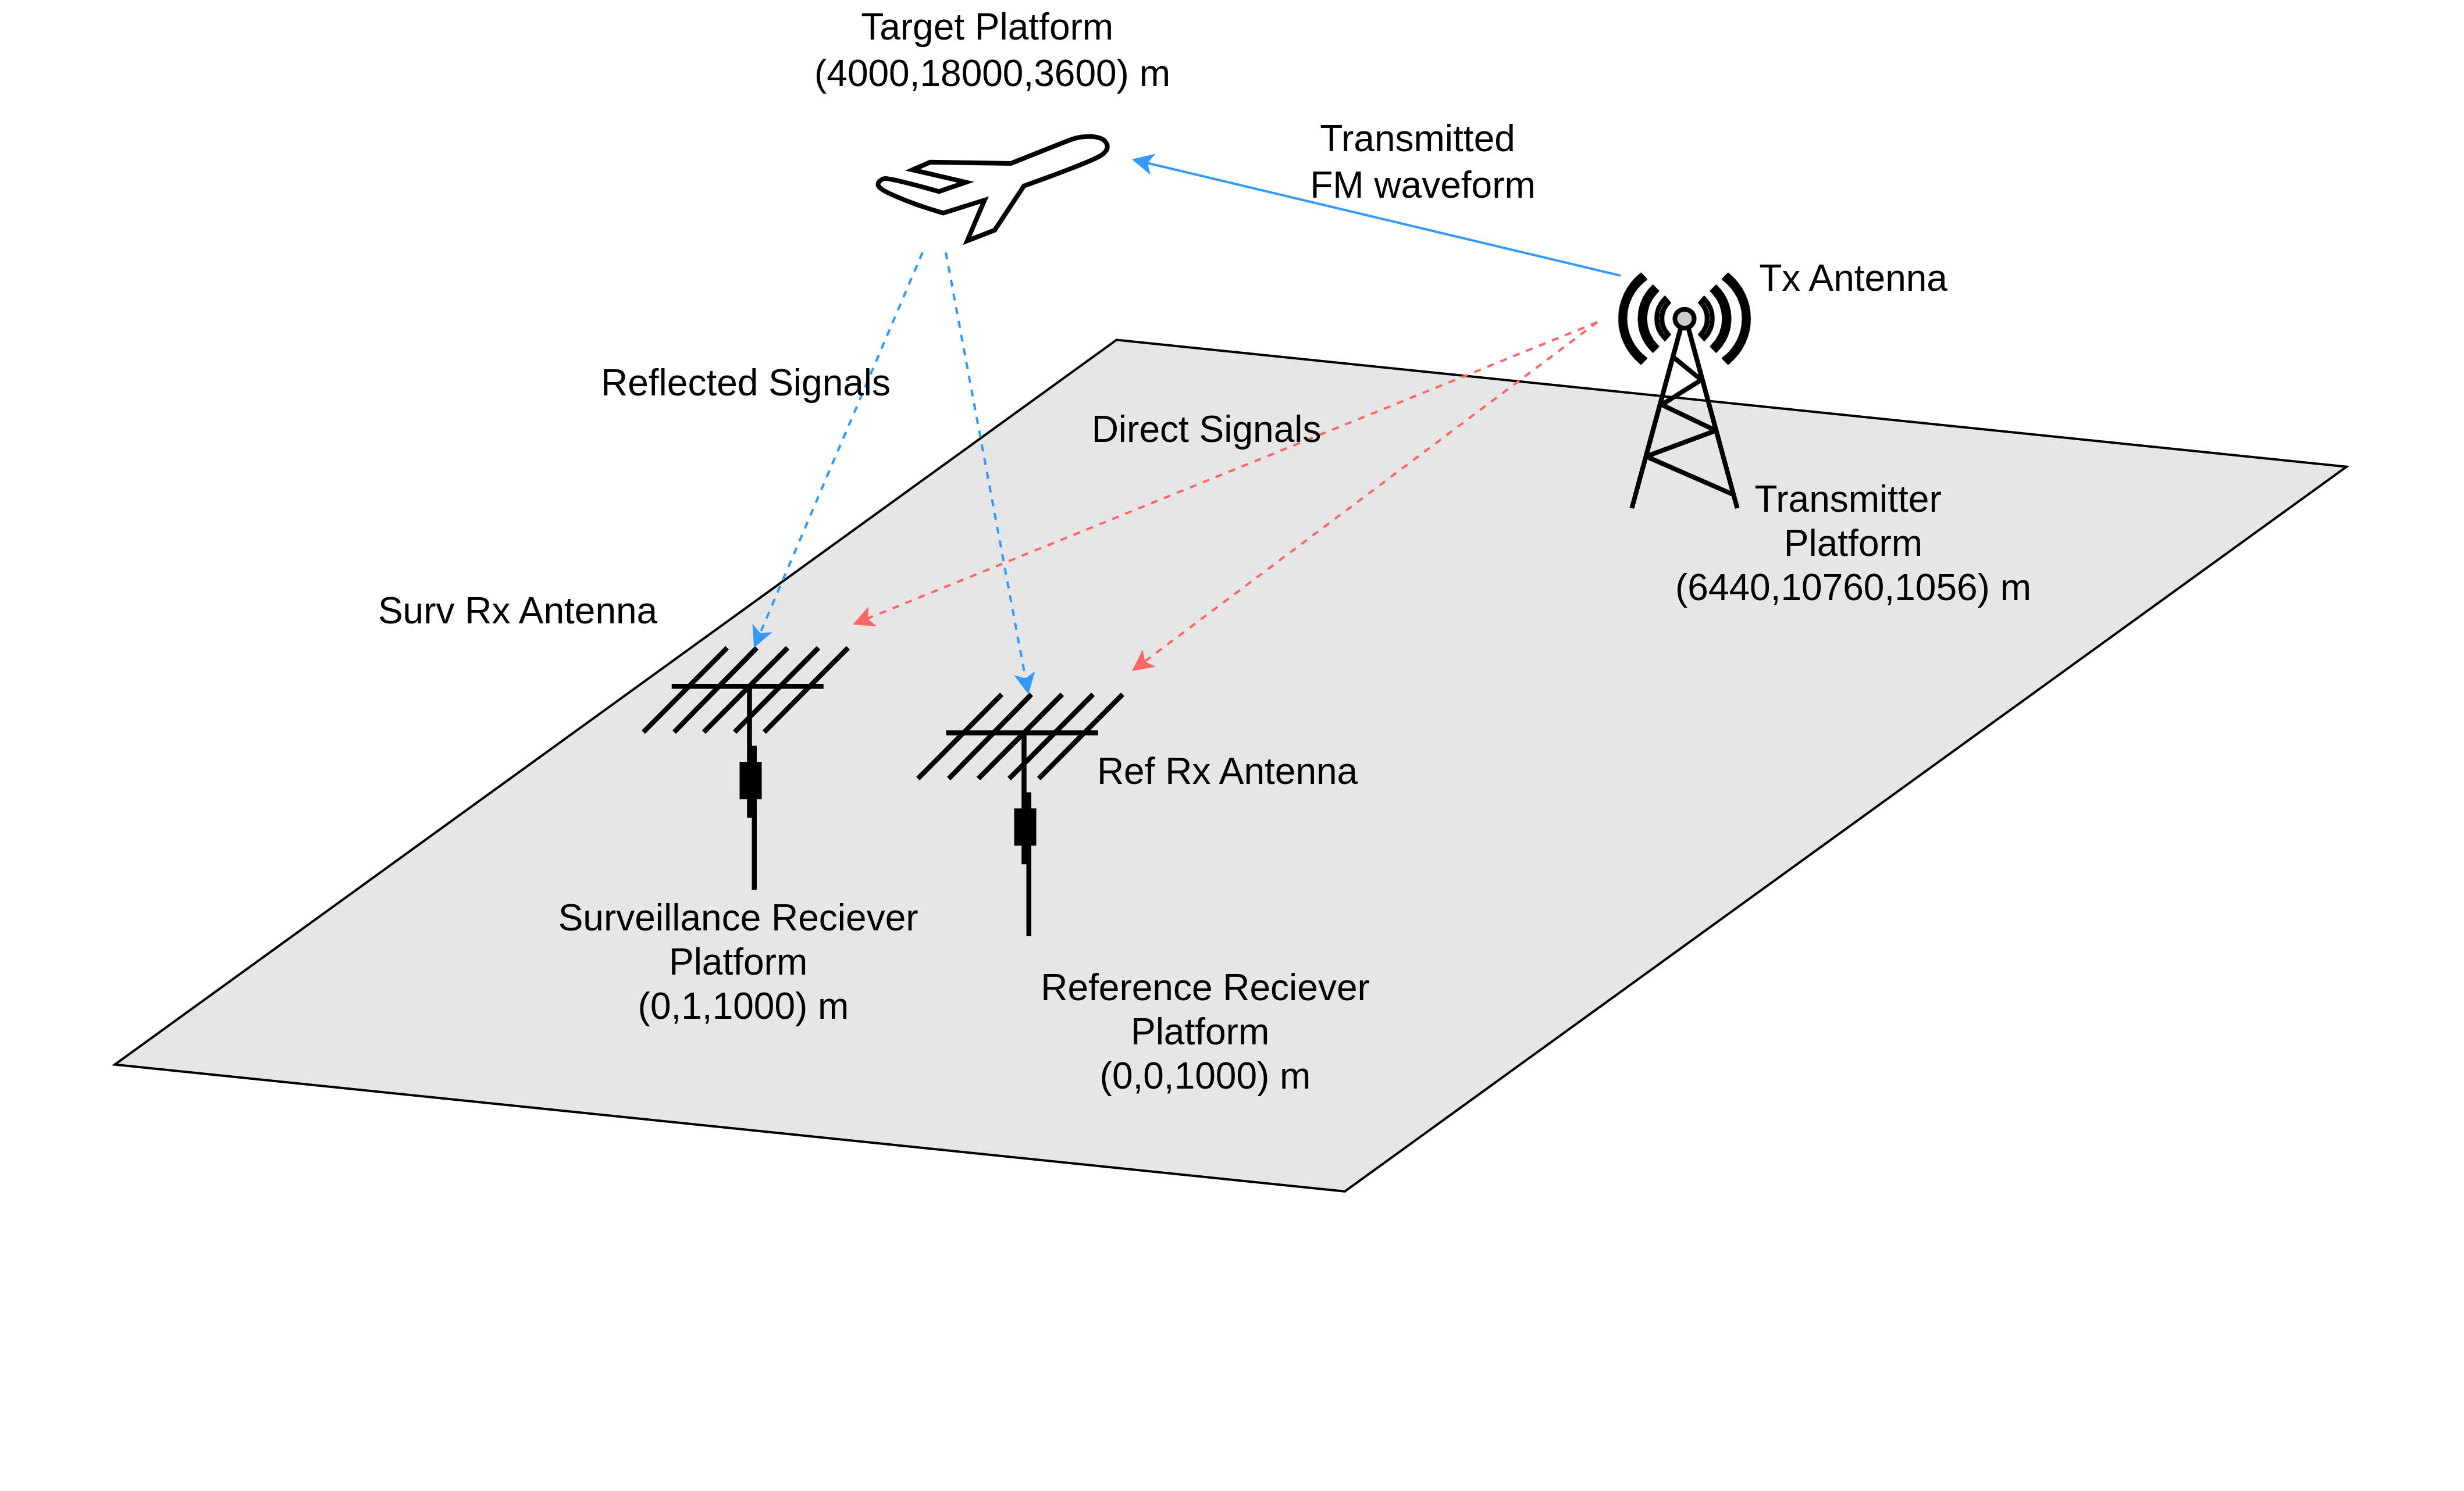
\includegraphics[width=0.85\linewidth]{Figure/fersBistaticRadar.drawio (3).png}
    \caption{Geometry of the Bistatic Radar in the FERS Simulation with the target in its initial position.}
    \label{fig:ferssetup}
\end{figure}
%%Corrections from Feeback [15]
The target is simulated as a single aircraft following a straight 
flight path, defined by Cartesian waypoints interpolated using cubic splines 
in MATLAB. The trajectory and corresponding ground truth data are shown in 
Figure \ref{fig:ard1setup}.
\newline
\begin{figure}[h!]
    \centering
    \begin{subfigure}[b]{0.49\linewidth}
        \centering
        \includesvg[width=\linewidth,inkscapelatex=false]{Figure/basicFersScenarioTargetPath.svg}
    \end{subfigure}
    \hfill
    \begin{subfigure}[b]{0.45\linewidth}
        \centering
        \includesvg[width=\linewidth,inkscapelatex=false]{Figure/basicFERS_ScenarioGroundTruth.svg}
    \end{subfigure}
    \caption{The basic FERS simulation scenario. Left: Target trajectory for 
    the straight and level flight scenario in Cartesian coordinates. Right: 
    Ground truth bistatic range and Doppler shift computed from the 
    simulated target coordinates at each time step.}
    \label{fig:ard1setup}
\end{figure}
%%%%%%%%%%%%%%%%%%%%%%%%%%%%%%%%%%%%%%
%%%%%%%%%%%%%%%%%%%%%%%%%%%%%%%%%%%%%%

The bistatic range and Doppler processing utilizes a set of 200 kilosamples, determined by the configured sampling rate in \ac{FERS}. The \ac{ARD} response output observed in Figure \ref{fig:ambiguityFunction} is taken after 2 seconds of sampling data. The resulting \ac{ARD} shown in Figure \ref{fig:ambiguityFunction}  exhibits a distinctive peak at a bistatic Doppler shift of 0 Hz. The peak at 0 Hz, strongest near zero range, indicates \ac{DPI}, likely due to signal leakage into the surveillance channel. Additional peaks at similar ranges to the \ac{DPI} are sidelobes of the \ac{FM} waveform's ambiguity function, further obscuring the target, it can be observed that the returns from the \ac{DPI} complicate target resolution.

\begin{figure}[H]
    \centering
    \includesvg[width=0.9\linewidth]{Figure/ardMapFinal.svg}
    \caption{Amplitude/Range/Doppler map.}
    \label{fig:ambiguityFunction}
\end{figure}
Although the cross-correlation function enhances processing gains, it also amplifies DPI and clutter which is undesired, leading to side-lobes that often mask target returns, as observed in Figure \ref{fig:ambiguityFunction}. The following subsection will discuss the application of a DPI cancellation algorithm for suppressing the \ac{DPI} and clutter.

%Range Smearing and side lobes

\subsection{Direct Path Interference and Clutter Suppression}
To improve the probability of detection, it is essential to suppress \ac{DPI} and clutter from the surveillance channel. This suppression is performed directly on the surveillance signal before the range and Doppler Processing stage. For this purpose, the \ac{ECA} which uses the least mean squares estimator technique is applied. The \ac{ECA}, as proposed by Colone \textit{et al.}\cite{coloneECA}, is recognized for its fast convergence and not requiring any tuning \cite{OHagan2008, tong2014}. Notably, in 2007 Cardinali \textit{et al.} conducted a comparative study of various \ac{DPI} cancellation algorithms, demonstrating the superior performance of the \ac{ECA} in achieving nearly complete clutter suppression, despite its higher computational demands compared to the other algorithms \cite{cardinali2007comparison,Heunis2010}. The \ac{ECA} is therefore selected for its proven effectiveness in mitigating clutter and \ac{DPI}. The focus here is on validating the results of this algorithm to ensure it operates as expected. The \ac{ARD} plot in \ac{2D} is shown before and after the DPI and clutter cancellation at \(t=2\)s in figures \ref{fig:ardDPIbefore} and \ref{fig:ardDPIAfter} respectively.

\begin{figure}[H]
    \centering
    \includesvg[width=0.8\linewidth,inkscapelatex=false]{Figure/ardBeforeDPI_unnormalized_correction1.svg}
    \caption{Amplitude/Range/Doppler map before DPI and clutter cancellation.}
    \label{fig:ardDPIbefore}
\end{figure}
\begin{figure}[H]
    \centering
    \includesvg[width=0.8\linewidth,inkscapelatex=false]{Figure/ardFinalAfter_correction1.svg}
    \caption{Amplitude/Range/Doppler map after DPI and clutter cancellation. The line at 0 Hz bistatic Doppler frequency indicates zero Doppler cancellation. The black circle marking illustrates the  target that  appears at a Doppler frequency of around 147 Hz.}
    \label{fig:ardDPIAfter}
\end{figure}

The range and Doppler map reveal the target more clearly after applying the \ac{ECA} algorithm, with the target observed at a bistatic Doppler frequency of around 147 Hz. Notably, the line at zero bistatic Doppler frequency shows a significantly reduced amplitude, illustrating the strong cancellation of zero Doppler components and demonstrating the effectiveness of the \ac{DPI} cancellation.

\subsection{Target Detection}
The Target Detection stage is responsible for identifying potential targets from the \ac{ARD} map. Using the range and Doppler response plots discussed in the previous subsections, this stage involves evaluating each cell in the range and Doppler domain against some threshold. This threshold is typically determined based on the values of the surrounding cells to effectively distinguish targets from background noise. One of the common effective implementations is the use of a \ac{CFAR} filter. This method provides the capability to tune the probability of detection \(p_d\) by varying the probability of false alarm \(P_{fa}\).


%Motivation for CA CFAR
In \ac{Radar} signal processing, various algorithms are designed for adaptive thresholding to achieve a \ac{CFAR}. 
These algorithms include, but are not limited to, \ac{CA-CFAR}, \ac{OSGO-CFAR}, \ac{VI-CFAR}, \ac{OS-CFAR}, \ac{SO-CFAR}, and \ac{GO-CFAR} \cite{hatem2018comparative}. In this research, the \ac{CA-CFAR} algorithm is used for target detection due to its simplicity and lower complexity compared to the other \ac{CFAR} algorithms. The \ac{CA-CFAR} has been effectively used in conjunction with similar algorithms used in this research, such as the \ac{ECA} for detection in \ac{PR} systems \cite{Colone2009,Golabi2013}.

\subsubsection{Cell-Averaging CFAR}
The \ac{CFAR} filter's function is to establish the power threshold, beyond which any detected echo is likely to be from a target. If this threshold is set too low, it will result in more echoes being detected, leading to an increase in false alarms \cite{Shrivathsa2008a}. In the \ac{CA-CFAR} case this is achieved by averaging the output over the adjacent cells to compute the threshold.
\begin{figure}[H]
    \centering
    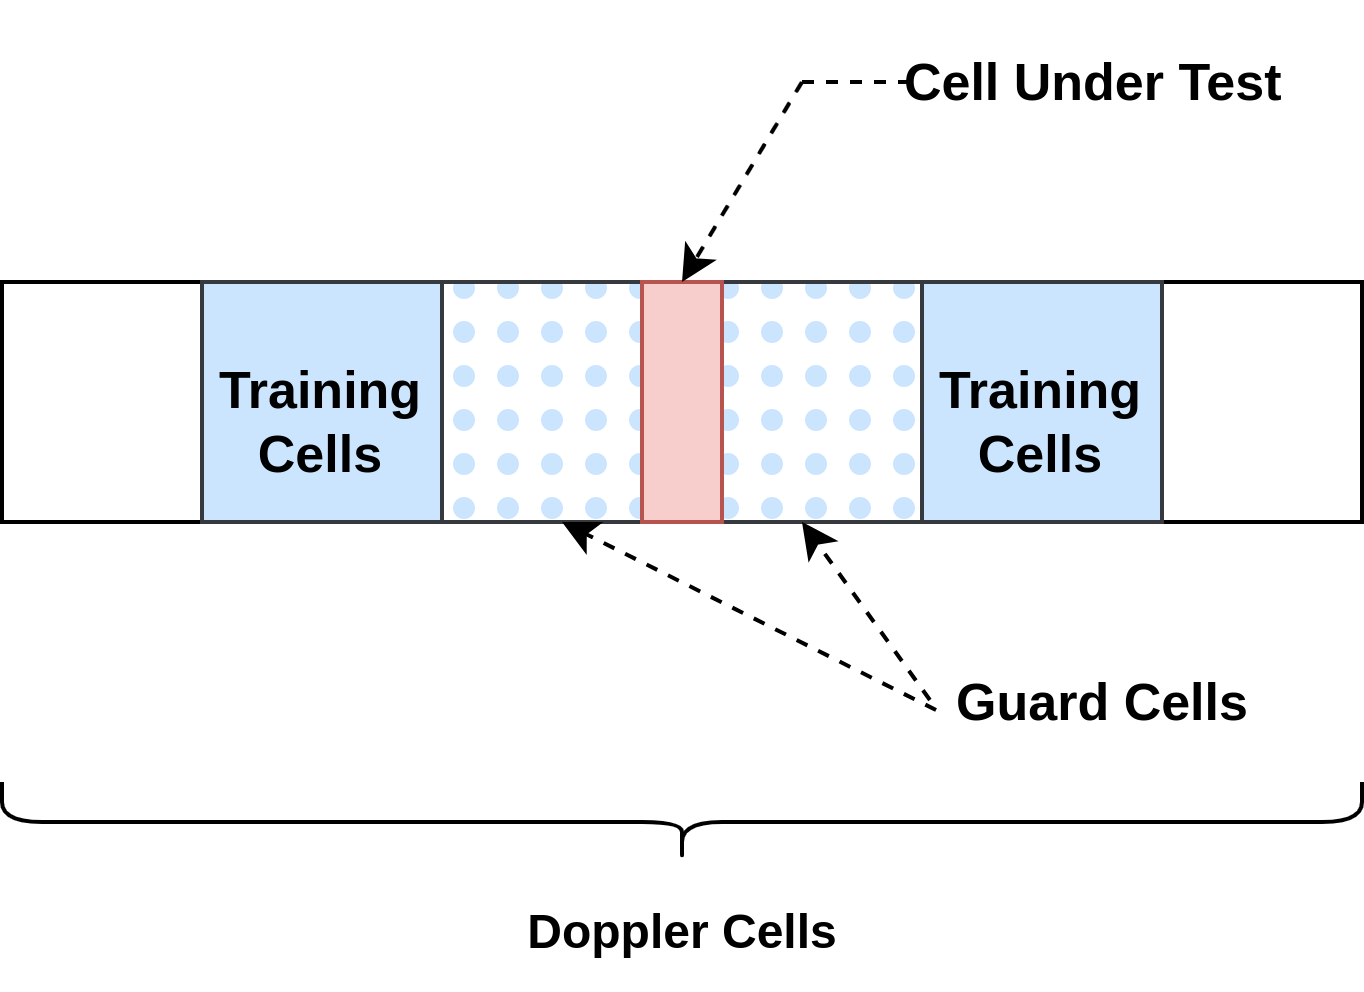
\includegraphics[width=0.55\linewidth]{Figure/cacfar.drawio.png}
    \caption{Cell-Averaging CFAR principle.}
    \label{fig:cacfar}
\end{figure}
%Norman Pearson Detector
The basic principle of the \ac{CA-CFAR} algorithm is illustrated in Figure \ref{fig:cacfar}. In this method, the adjacent cells to the \ac{CUT} are designated as guard cells. The selection of these guard cells depends on the expected number of cells to be occupied by the target in the range or Doppler domain, which is influenced by the \ac{Radar}’s resolution capabilities. Training cells, located around the \ac{CUT}, are used to dynamically compute the average noise power. This average is then scaled by a factor \(\alpha\) to determine the threshold for target detection, as shown in Equation (\ref{thresholdCFAR}). If the power level in the \ac{CUT} exceeds this threshold, a target is detected.

The noise power \(P_n\) from the neighboring cells is scaled by the factor \(\alpha\) \cite{Shrivathsa2008a}:
\begin{equation}
    T = \alpha \cdot P_n
    \label{thresholdCFAR}
\end{equation}

To compute \(P_n\) the  power levels from the training cells are averaged, where \(x_m\) represents the power level in the \(m\)-th cell and \(N\) is the number of training cells as shown in Equation (\ref{thresholdCFAR}):

\begin{equation}
    P_n = \frac{1}{N} \sum_{m=1}^N x_m
\end{equation}
\newline
\newline
The scaling factor is computed according to Equation (\ref{alpha}) where \(P_{fa}\) is the desired probability of false alarm  \cite{Sambath2020a} :

\begin{equation}
    \alpha = N \cdot (P_{fa}^{-\frac{1}{N}}-1)
    \label{alpha}
\end{equation}
%NB - make other references to range smearing
In the range and Doppler plots discussed in the previous subsection, it is observed that the target spans across multiple range bins. This is a common issue when using \ac{FM} transmitted waveform due to low bandwidth, coupled with the instantaneous bandwidth due to the inconsistencies in the broadcasted audio signal, which can cause fluctuations in the range resolution (\(\delta R = c/2B\)), leading to range smearing. This makes setting the number of guard and reference cells in range dimension challenging. Consequently, averaging is then performed only in the bistatic Doppler domain, where higher Doppler resolution is available. The \ac{CA-CFAR} parameters used are presented in Table \ref{tab:cacfartable}.

\begin{table}[ht!]
\centering
\caption{CA-CFAR Parameters.}
\label{tab:cacfartable}
\begin{tabular}{ll}
\hline
\textbf{Parameter} & \textbf{Value} \\
\toprule
\(P_{fa}\)  & \(10^{-5}\) \\
Doppler Training Cells & 6  \\
Doppler Guard Cells  & 4 \\
\bottomrule
\end{tabular}
\end{table}
 The \(P_{fa}\)  was selected through a systematic sensitivity analysis, the results of which are illustrated in Figure~\ref{fig:cfarValidation}, which presents a range-Doppler line cut at a bistatic range of 15~km. Lower \(P_{fa}\)  values produced thresholds approaching the noise floor, increasing susceptibility to false alarms, while higher values elevated the threshold above the target return, risking target suppression. A \(P_{fa}\) value of \(10^{-5}\)  was therefore selected as it provided the most favourable balance between detection sensitivity and false alarm suppression. The \ac{CA-CFAR} was used with 4 guard cells and 6 training cells on both sides of the \ac{CUT}, similar to the approach followed in \cite{De2015,tong2014}. Figure \ref{cfarwindow} shows the CFAR window.
\newline
\begin{figure}[H]
    \centering
    \includesvg[width=1\linewidth]{Figure/cfar_ca.drawio.svg}
    \caption{CFAR window with 21 cells.}
    \label{cfarwindow}
\end{figure}
Using the parameters listed in Table \ref{tab:cacfartable}, the \ac{CA-CFAR} is applied on the range and Doppler map and the output is shown in Figure \ref{fig:ca-cfar1}.
%false alarm ??
\begin{figure}[H]
    \centering
    \includesvg[width=0.7\linewidth,inkscapelatex=false]{Figure/cacfar_pfa5_corrections.svg}
    \caption{CA-CFAR output with \(P_{fa}\) of \(10^{-5}\): The Target is observed at around a bistatic Doppler frequency of 147 Hz.}
    \label{fig:ca-cfar1}
\end{figure}

\begin{figure}[H]
    \centering
    \includesvg[width=0.7\linewidth,inkscapelatex=false]{Figure/cacfar_pfa7_correction.svg}
    \caption{CA-CFAR output with \(P_{fa}\) of \(10^{-7}\): A decrease in the number of observations is observed due to the decrease in \(P_{fa}\).}
    \label{fig:ca-cfar2}
\end{figure}

To validate the accuracy of the dynamic threshold and the functionality of the \ac{CA-CFAR} filter, the bistatic Doppler response and the threshold are computed at a specific bistatic range with different \(P_{fa}\) where the target is present, as shown in Figure \ref{fig:cfarValidation}.

\begin{figure}[H]
    \centering
    \includesvg[width=0.9\linewidth,inkscapelatex=false]{Figure/ca_cfar_validate_corrections_v2.svg}
    \caption{CA-CFAR output with the threshold value at a bistatic range of 15 km with a \(P_{fa}\) of \(10^{-3}\) to \(10^{-7}\).}
    \label{fig:cfarValidation}
\end{figure}



\subsubsection{Target  Centroids}
The \ac{CFAR} outputs presented in the previous subsection, show multiple detections across various  Doppler and range cells. To effectively use these detections in tracking filters, additional processing is necessary to group the detections into clusters and extract target coordinates. Each cluster represents a distinct target, and the extracted centroids will serve as measurements for tracking filters. Identifying distinct targets from a \ac{CFAR} output usually involves a robust clustering algorithm to group the bistatic range and Doppler cells associated with each target.

Various clustering techniques have been used throughout the literature for post-processing CFAR detections. For instance, in \cite{kuang2020applied}, the K-means clustering algorithm is used to derive target centres from \ac{CFAR} outputs. Additionally, \ac{DBSCAN} has been used to identify clusters in \ac{CFAR} detections, as demonstrated in \cite{li2024density,schubert2015clustering}. Mean-shift clustering, a well-known density-based method, differs from K-means in that it does not require prior knowledge of the number of clusters or assumptions about their shapes. While \ac{DBSCAN} can identify clusters, additional processing is required to compute the mean of the points in each cluster to extract the centroids. In contrast, mean-shift clustering relies solely on an estimated bandwidth size to group detections, as outlined in \cite{derpanis2005mean}. Consequently, the mean-shift algorithm is used here to directly produce target centroids from \ac{CFAR} outputs.
\newline
\newline
%Clustering
Mean-shift clustering is an iterative algorithm that shifts each data point toward regions of higher density in the feature space \cite{cheng1995mean}. It does so by moving each point to the mean of points within a specified bandwidth. This process continues until convergence, forming clusters as points gather around high-density regions. The kernel used, typically a Gaussian kernel, determines how weights are applied within the bandwidth, influencing the direction and magnitude of the shift \cite{cariou2022novel}. This results in a set of cluster centroids representing the densest areas in the data. The mean-shift clustering algorithm is discussed extensively in the literature \cite{cariou2022novel,wu2007mean}, with the focus here being on validating its results. The algorithm used is illustrated in algorithm \ref{alg:mean_shift}, adapted from \cite{carreira2015review}. 
\newline 
\newline
\begin{figure}[H]
    \centering
    \includesvg[width=0.7\linewidth,inkscapelatex=false]{Figure/cacfar_pfa7_centroid_correction.svg}
    \caption{CFAR output with centroids.}
    \label{fig:cfar_centers}
\end{figure}
The bandwidth parameter used in the mean-shift clustering algorithm for the bistatic Doppler and bistatic range measurements is selected as \( \sigma = [5 \, \text{Hz}, 10 \, \text{km}] \) respectively. Detections falling within this kernel bandwidth are considered part of the same neighbourhood. This parameter defines the neighbourhood size around each data point used for calculating the mean shift \cite{Wu2007}. Figure \ref{fig:cfar_centers} shows the clusters detected in the \ac{CFAR} output, with the centroids of each cluster highlighted as red squares. A drawback of this approach is that if target detections are closely spaced in both bistatic range and Doppler, they may be clustered into a single detection.\footnote{A video showing the \ac{CA-CFAR} with a \(P_{fa}\) of \(10^{-5}\) and Mean-Shift clustering outputs for a single target can be found at: \url{https://youtu.be/nWzsm2Biv8Y}. The Matlab code for the implementation of Mean-shift Algorithm and the \ac{CA-CFAR} can be found in the code repository from Appendix \ref{appendix:repo}.}
\newline 
\begin{algorithm}[H]
\caption{Mean-shift Clustering}
\label{alg:mean_shift}
\begin{algorithmic}[1]
    \vspace{2em}
    \State \textbf{Initialize:}
    \vspace{0.3em}
    \Statex $\text{dataPoints} \gets \text{input data}$
    \Statex $\text{bandWidthX} \gets \text{bandWidthX}$
    \Statex $\text{bandWidthY} \gets \text{bandWidthY}$
    \Statex $\text{stopThresh} \gets 1e{-3} \times [\text{bandWidthX}, \text{bandWidthY}]$
    \Statex $\text{clusterCentroids} \gets [\,]$
    \vspace{1em}
    
    \State \textbf{Main Loop:}
    \vspace{1em}
    \While{$\text{numInitPts} > 0$}
        \State $\text{startPt} \gets \text{randomly select a point from initial Points}$
        \State $\text{mean} \gets \text{dataPoints[:, startPt]}$
        \vspace{0.5em}
        \While{not converged}
            \State $\text{sqDistToAll} \gets \frac{(\text{mean}(1)-\text{dataPoints}(1,:))^2}{\text{bandWidthX}} + \frac{(\text{mean}(2)-\text{dataPoints}(2,:))^2}{\text{bandWidthY}}$
            \vspace{0.5em}
            \State $\text{weights} \gets \exp\left(-\frac{1}{2} \times \text{sqDistToAll}\right)$
            \vspace{0.5em}
            \State $\text{newMean} \gets \frac{\sum (\text{weights} \times \text{dataPoints}[:, :])}{\sum \text{weights}}$
            \vspace{0.5em}
            \State $\text{Members} \gets [\text{Members}, \text{find}(\text{sqDistToAll} < 1)]$
            \vspace{0.5em}
            \State $\text{beenVisitedFlag}[\text{Members}] \gets 1$
            \vspace{0.5em}
            \If{$\text{norm}(\text{newMean} - \text{mean}) < \text{stopThresh}$}
                \State Check for merge possibilities
                \vspace{0.5em}
                \If{merge found}
                    \State Merge clusters
                \Else
                    \State Create new cluster
                \EndIf
                \State \textbf{break}
            \EndIf
            \vspace{0.5em}
            \State $\text{mean} \gets \text{newMean}$
        \EndWhile
        \vspace{0.5em}
        \State \text{Update clusters and initial Points}
    \EndWhile
    \vspace{1em}
\end{algorithmic}
\end{algorithm}

\newpage
\section{Target Modelling}

The centroids from the clustering process, are used to estimate the target's position in the bistatic range and Doppler domain. To accurately estimate the target's state, it is required to model the target's motion. Target motion models are typically classified as either manoeuvring or non-manoeuvring  in tracking problems \cite{Li2003a}. For our tracking scenarios, a non-maneuvering target, such as a commercial aircraft, is expected in the bistatic Doppler and range domain, where abrupt changes in the bistatic range or Doppler are unlikely. Therefore, a \ac{NCV} model is used, similar to \cite{Boyer2012} which assumes a nearly constant velocity between the sampling interval.

\subsection{Nearly-Constant Velocity Model}
The target's motion in a \ac{2D} Cartesian coordinate system with constant velocity can be modelled by the state vector \( [x, \dot{x}, y, \dot{y}] \), where \( x \) and \( y \) represent positions, and \( \dot{x} \) and \( \dot{y} \) represent velocities. Similarly, the state of the target in the bistatic range and Doppler domain is modelled by the bistatic range, bistatic range rate, bistatic Doppler, and bistatic Doppler rate, as shown in  Equation (\ref{stateEq}):

\begin{equation}
    x(t) = [r_t, \dot{r}, f_t, \dot{f_t}]^T
    \label{stateEq}
\end{equation}

where \(r_t\) is the bistatic range, \(f_t\) is the bistatic Doppler, \(\dot{r_t}\) and \(\dot{f_t}\) are bistatic range rate and bistatic Doppler rate respectively in continuous time. The \ac{NCV} model is represented as:

\begin{equation}
    \mathbf{X}_k = 
    \begin{bmatrix}
        1 & \tau & 0 & 0 \\
        0 & 1 & 0 & 0 \\
        0 & 0 & 1 & \tau \\
        0 & 0 & 0 & 1 \\
    \end{bmatrix} X_{k-1} + w_{k-1}
\end{equation}

where, \( \tau \) is the sampling interval, and \( w_{k-1} \) is the discrete white acceleration noise. This noise accounts for small, random variations in acceleration that cannot be predicted \cite{Li2003a}. Assuming a discrete-time model with zero-mean white Gaussian noise characterized by the covariance matrix \( Q \):

\begin{equation}
    Q = \text{cov}(w_k) = S_w \tilde{Q},
\end{equation}

where:

\begin{equation}
    \tilde{Q}  = \begin{bmatrix}
        \tau^4/4 & \tau^3/2 & 0 & 0 \\
        \tau^3/2 & \tau^2 & 0 & 0 \\
        0 & 0 & \tau^4/4 & \tau^3/2\\
        0 & 0 & \tau^3/2 & \tau^2\\
    \end{bmatrix}
    \label{Qmatrix}
\end{equation}

\( S_w \) represents the process noise power spectral density \cite{Measurements2023b}. The white acceleration model can also be adapted for tracking manoeuvring targets by using the manoeuvring index \( \lambda \) defined as:

\begin{equation}
    \lambda = \frac{\sqrt{S_w \tau^3}}{\sigma_r}, 
\end{equation}

where \( \lambda \) is the ratio of the \ac{RMS} motion uncertainty to the measurement uncertainty. Lower values of \( S_w \) describe a \ac{NCV} model, while higher values correspond to a manoeuvring target model \cite{953264}.


\section{Tracking Filters Implementation}

This section describes the implementation of the tracking filters introduced in Chapter 3. The filters are used to track targets based on observations from the target detections. A basic scenario with a simulated target in the FERS framework is used to demonstrate the functionality of the four filters. The target is simulated in the same bistatic radar geometric setup 
from Figure \ref{fig:ferssetup}. The trajectory and corresponding ground 
truth data are shown in Figures \ref{fig:targetpath2} and 
\ref{fig:groundtruth2} respectively. The performance and investigation of 
the filters' optimal parameters are discussed in the next chapter.

\begin{figure}[H]
    \centering
    \includesvg[width=0.7\linewidth,inkscapelatex=false]{Figure/basicFersScenarioTargetPath2.svg}
    \caption{Target trajectory for the flight scenario in Cartesian 
    coordinates.}
    \label{fig:targetpath2}
\end{figure}

\begin{figure}[H]
    \centering
    \includesvg[width=0.55\linewidth,inkscapelatex=false]{Figure/basicFERS_ScenarioGroundTruth2.svg}
    \caption{Ground truth bistatic range and Doppler shift computed from 
    the simulated target coordinates at each time step.}
    \label{fig:groundtruth2}
\end{figure}%feedback 15
\subsection{Kalman Filter}
The Kalman Filter is implemented using the algorithm shown in Algorithm \ref{alg:kalman_filter}. The parameters that need to be initialized include the initial state estimate \(x_0\), the initial error covariance matrix \(P_0\), the process noise covariance matrix \(Q\), and the measurement noise covariance matrix \(R\). The first detection of the target is used to initialize the state vector \(x_0\).

\textbf{Initial Error Covariance Matrix:}
\newline
The initial error covariance matrix, as discussed in Section 3, models the uncertainty in the state estimate. The error covariance matrix is updated in each prediction-update cycle of the Kalman Filter. It is initialized according to the expected uncertainty values, similar to the approach followed by Howland \cite{Howland2005a}:
\begin{equation}
    P_0 = \begin{bmatrix}
        5 & 0 & 0 & 0 \\
        0 & 0.04 & 0 & 0 \\
        0 & 0 & 0.0225 & 0 \\
        0 & 0 & 0 & 0.1 \\
    \end{bmatrix}
\end{equation}


\textbf{Measurement Error Covariance Matrix:}
\newline
The measurement error covariance matrix, defined in Equation (\ref{measurement_eq}), is selected based on the expected standard deviation of the measurement errors in the bistatic range and Doppler domains:

\begin{equation}
    R = \begin{bmatrix}
        \sigma_{\text{range}}^2 & 0 \\
        0 & \sigma_{\text{doppler}}^2 \\
    \end{bmatrix}
\end{equation}

The measurement covariance matrix values were determined by analysing the observed deviations in the bistatic range and Doppler domain. The bistatic range standard deviation, \(\sigma_{\text{range}} = 1\) km, was obtained from the standard deviation of errors between simulated and ground truth data. Similarly, the Doppler shift standard deviation, \(\sigma_{\text{doppler}} = 0.1\) Hz, was obtained from observed deviations in Doppler measurements. This approach aligns with \cite{De2015}, where standard deviations from field deployment data were used to define the measurement covariance matrix.  

\textbf{Process Noise Covariance Matrix:}
\newline
The process noise covariance matrix is defined by the Equation in (\ref{Qmat}), where \(S_w = [s_{w1}, s_{w2}]\) represents the process noise power spectral densities for the bistatic range and Doppler, respectively:
\begin{equation}
    Q  = \begin{bmatrix}
        \frac{\tau^4}{4} s_{w1} & \frac{\tau^3}{2} s_{w1} & 0 & 0 \\
        \frac{\tau^3}{2} s_{w1} & \tau^2 s_{w1} & 0 & 0 \\
        0 & 0 & \frac{\tau^4}{4} s_{w2} & \frac{\tau^3}{2} s_{w2} \\
        0 & 0 & \frac{\tau^3}{2} s_{w2} & \tau^2 s_{w2} \\
    \end{bmatrix}
    \label{Qmat}
\end{equation}

The values of \(s_{w1}  \) and \(s_{w2}\) are determined through a tuning process and their effect is demonstrated in Figure \ref{kalman_results1}.
\begin{figure}[H]
    \centering
    \begin{subfigure}[b]{0.49\linewidth}
        \centering
        \includesvg[height=6cm,inkscapelatex=false]{Figure/kf_R_corrections_v1.svg}
        \caption{Kalman Filter with different values for \(\sigma_{range}\) and \(\sigma_{doppler}\).}
        \label{kalman_results}
    \end{subfigure}
    \hfill
    \begin{subfigure}[b]{0.49\linewidth}
        \centering
        \includesvg[height=6cm,inkscapelatex=false]{Figure/kf_SW_corrections_v1.svg}
        \caption{Kalman Filter with different values for \(s_{w1}\) and \(s_{w2}\) for the \(Q\) covariance matrix.}
        \label{kalman_results1}
    \end{subfigure}
    \caption{ Kalman Filter with varying measurement and process noise covariance matrices.}
\end{figure}

A single target is configured in \ac{FERS} using the geometric setup in Figure \ref{fig:ferssetup} and the target path in Figure \ref{fig:targetpath2}. The results for the basic scenario in \ac{FERS} using the Kalman Filter are presented in figures \ref{kalman_results} and \ref{kalman_results1}.
\newline
% Added cumulative error metric and two new figures
\begin{figure}[H]
    \centering
    \begin{subfigure}[b]{0.49\linewidth}
        \centering
        \includesvg[width=\linewidth,inkscapelatex=false]{Figure/KF_R_CumSum.svg}
        \caption{Kalman Filter Cumulative Error with different values for \(\sigma_{range}\) and \(\sigma_{doppler}\).}
        \label{kalman_results_cum}
    \end{subfigure}
    \hfill
    \begin{subfigure}[b]{0.49\linewidth}
        \centering
        \includesvg[width=\linewidth,inkscapelatex=false]{Figure/KF_Q_CumSum.svg}
        \caption{Kalman Filter Cumulative Error with different values for \(s_{w1}\) and \(s_{w2}\) for the \(Q\) covariance matrix.}
        \label{kalman_results_cum1}
    \end{subfigure}
    \caption{ Kalman Filter Cumulative Error with varying measurement and process noise covariance matrices.}
\end{figure}
To provide a quantitative assessment of the sensitivity of the Kalman Filter to the covariance matrices $\mathbf{R}$ and $\mathbf{Q}$, a cumulative error metric was computed relative to the ground truth trajectory. The cumulative error is defined as the sum of the Euclidean distance between the estimated and true target positions over the duration of the simulation. The resulting cumulative errors for different parameter configurations are shown in Figures \ref{kalman_results_cum} and \ref{kalman_results_cum1}.

The behaviour of a tracking filter is highly influenced by the process noise covariance matrix $\mathbf{Q}$ and the measurement noise covariance matrix $\mathbf{R}$. As shown in Figure \ref{kalman_results}, increasing the values in $\mathbf{R}$ results in less precise predictions, with the filter giving more weight to the process model rather than the measurements. This leads to predictions that are more loosely constrained, as expected. Similarly, Figure \ref{kalman_results1} demonstrates the impact of increasing the process noise power spectral density. The cumulative error results shown in Figures \ref{kalman_results_cum} and \ref{kalman_results_cum1} also provide a quantitative confirmation of these effects. Higher values lead to a larger process noise covariance matrix, causing the predicted state estimates to become more dispersed, reflecting the increased uncertainty in the system's dynamics. This confirms the significant impact that both the $\mathbf{R}$ and $\mathbf{Q}$ covariance matrices have on estimating dynamic states as noted in \cite{Akhlaghi2018}.



\subsection{Unscented Kalman Filter}
Similar to the Kalman Filter, the matrices \(P\), \(R\), \(Q\), and the state vector \(x_0\) are initialized in the same way. However, additional parameters are required for the \ac{UKF}, as shown in Table \ref{tab:ukf_params}.
\begin{table}[H]
    \centering
    \large
    \caption{Parameters Used for Unscented Kalman Filter.}
    \label{tab:ukf_params}
    \begin{tabular}{ll}
        \toprule
        Parameter & Value \\
        \midrule
        \( n \) & 4 \\
        \( \alpha \) & 0.01 \\
        \( \kappa \) & 0 \\
        \( \beta \) & 2 \\
        \bottomrule
    \end{tabular}
\end{table}
The \ac{UKF} includes parameters \(\alpha\), \(\beta\), \(\kappa\), and \(n\), where \(\alpha\) controls the dispersion of sigma points relative to the state vector's mean, 
\(\kappa\) functions as an additional scaling factor, and \(\beta\) integrates prior information 
about the input random variable's distribution \cite{Cai2006}. The parameter \(n\) represents the dimension of the state vector. The value of \(\beta\) is typically chosen as 2, which is considered optimal, and \(\kappa\) is usually set to 0 \cite{Cai2006}. \(\alpha\) is generally set to a small value such as \(1 \times 10^{-3}\), and in this case, it was determined by varying the parameter and observing its impact, as demonstrated in Figure \ref{tab:ukf_params}.
 \newline
 \newline
The results of the \ac{UKF} tracking are presented in \ref{ukfres} and \ref{ukfres2} where different \ac{UKF} parameters for \(\alpha\) and \(\beta\) were used.
\begin{figure}[ht!]
    \centering
    \begin{subfigure}[b]{0.48\linewidth}
        \centering
        \includesvg[height=6cm,inkscapelatex=false]{Figure/ukf_alpha_v3.svg}
        \caption{UKF with different values for alpha.}
        \label{ukfres}
    \end{subfigure}
    \hfill
    \begin{subfigure}[b]{0.48\linewidth}
        \centering
        \includesvg[height=6cm,inkscapelatex=false]{Figure/ukf_beta_v3.svg}
        \caption{UKF with different values for beta.}
        \label{ukfres2}
    \end{subfigure}
    \caption{UKF with varying values of \(\alpha\) and \(\beta\).}
\end{figure}
As shown in Figure \ref{ukfres}, the impact of the \(\alpha\) parameter on the filter's estimations is evident. This is consistent with the role of \(\alpha\), which affects how the sigma points are spread around the mean of the state vector \cite{Cai2006}. For smaller values of \(\alpha\), the mean state estimate becomes more dispersed, leading to noticeable deviations in the filter estimates. As expected, the \(\beta\) parameter does not show any observable effect on the filter's estimations due to its minimal impact on the performance of the filter.
\newline
%%%%%%%%% Added cumulative error metric and two new figures %%%%%%%%%%%%
\begin{figure}[ht!]
    \centering
    \begin{subfigure}[b]{0.48\linewidth}
        \centering
        \includesvg[width=\linewidth,,inkscapelatex=false]{Figure/UKF_AlphaCumError.svg}
        \caption{\ac{UKF} Cumulative Error with different values for alpha.}
        \label{ukfresCumError}
    \end{subfigure}
    \hfill
    \begin{subfigure}[b]{0.48\linewidth}
        \centering
        \includesvg[width=\linewidth,inkscapelatex=false]{Figure/UKF_Beta_CumError.svg}
        \caption{\ac{UKF} Cumulative Error with different values for beta.}
        \label{ukfresCumError2}
    \end{subfigure}
    \caption{\ac{UKF} Cumulative Error with varying values of \(\alpha\) and \(\beta\).}
\end{figure}

The cumulative error results shown in Figures \ref{ukfresCumError} and \ref{ukfresCumError2} provide a quantitative measure of these effects. The results confirm that variations in the \(\alpha\) parameter influence the accumulated tracking error, reflecting the sensitivity of the UKF to the sigma point spread. In contrast, the cumulative error remains unchanged for different values of \(\beta\), indicating that this parameter has minimal influence on the filter performance in the considered scenario.
%%%%%%%%%%%%%%%%%%%%%%%%%%%%%%%%%%%%%%%%%%%%%%%%%%%%%%%%%%%%%%%%%%%%%%%%%%%%%
\subsection{Particle Filter}
The \ac{PF} has parameters such as the number of particles, the method of generating the particles on initialization, and the same \(R\), \(Q\), and \(x_0\) matrices used in the \ac{UKF} and Kalman Filter. The \ac{PF} is initialized with \(10,000\) particles, and a Gaussian \ac{PDF} is used to generate the particles upon track initialization. The results of the \ac{PF} with different numbers of particles are shown in Figure \ref{fig:particle_filter_results}.
\begin{figure}[H]
    \centering
    \includesvg[width=0.65\linewidth,inkscapelatex=false]{Figure/particles_corrections_v1.svg}
    \caption{Particle Filter output with a varying number of particles.}
    \label{fig:particle_filter_results}
\end{figure}
%%%%%%%% Added cumulative error metric and one new figures %%%%%%
To further quantify the effect of the number of particles on the filter performance, the cumulative tracking error metric is evaluated for different number of particles. The resulting cumulative errors are presented in Figure \ref{fig:particle_filter_cum_error}. The number of particles directly affects the accuracy of the filter's outputs. Using more particles provides a better approximation of the posterior distribution, leading to more accurate state estimates and reduced variance. Conversely, using too few particles can result in noisier outputs and less reliable tracking.
\begin{figure}[ht!]
    \centering
    \includesvg[width=0.6\linewidth,inkscapelatex=false]{Figure/PF_ParticlesCumError.svg}
    \caption{Particle Filter cumulative error for different numbers of particles.}
    \label{fig:particle_filter_cum_error}
\end{figure}
%%%%%%%%%%%%%%%%%%%%%%%%%%%%%%%%%%%%%%%%%%%%%%%%%%%%%%%%%%%%%%%%%%%
 The effect of different numbers of particles is demonstrated in Figure \ref{fig:particle_filter_results} and further confirmed by the cumulative error results in Figure \ref{fig:particle_filter_cum_error}, which show a clear reduction in accumulated tracking error as particle count increases. This behaviour is consistent with the findings reported in \cite{Bauermeister2016}. This aligns with findings from \cite{Bauermeister2016}, which showed that the \ac{SIR} Particle Filter's accuracy is influenced by the number of particles used.

\subsection{RGNF Filter}
The \ac{RGNF} filter has only additional parameters compared to the other filters, such as \(\lambda\), which is discussed in the theory section as the forgetting factor. Other parameters are the maximum number of iterations and the tolerance. The parameters used are shown in Table \ref{tablergnf}.

\begin{table}[H]
    \centering
    \caption{Parameters for the RGNF Filter.}
    \label{tablergnf}
    \begin{tabular}{c|c}
        \toprule
        Parameter & Value \\
        \midrule
        \( \lambda \) & 0.9 \\
        Max Iterations & 100 \\
        Tolerance & 1e-3 \\
        \bottomrule
    \end{tabular}
\end{table}

The parameter \(\lambda\) significantly influences the performance of the \ac{RGNF} in contrast to the other parameters, serving as the filter's memory length. It is important to observe its effect, as lower values of \(\lambda\) are expected to yield a more dynamic estimation behaviour and larger values to produce more robust estimations and cause the filter to behave similarly to a Kalman Filter, as demonstrated by Roaldje \cite{Nadjiasngar2012}. 
\begin{figure}[H]
    \centering
    \includesvg[width=0.7\linewidth,inkscapelatex=false]{Figure/rgnf_results}
    \caption{RGNF tracking filter output with different values of \(\lambda\).}
    \label{fig:rgnf_results}
\end{figure}
%%%%%%%%%%%% Cumulative Error Section %%%%%%%%%%%%%%%%%%%%%
Figures \ref{fig:rgnf_results} and \ref{fig:rgnf_cum_error} confirm this behaviour, with \(\lambda = 1\) yielding the largest accumulated error due to the filter's reduced adaptability. An intermediate value of \(\lambda = 0.9\) was therefore selected, as it provides an optimal balance between measurement responsiveness and estimation stability.

\begin{figure}[H]
    \centering
    \includesvg[width=0.6\linewidth,inkscapelatex=false]{Figure/RGNF_LambdaCumError.svg}
    \caption{RGNF cumulative error for different values of \(\lambda\).}
    \label{fig:rgnf_cum_error}
\end{figure}

%%%%%%%%%%%%%%%%%%%%%%%%%%%%%%%%%%%%%%%%%%%%%%%%%%%%%%%%%%%%%%%%%%%%

\subsection{Multi-Target Tracking}
The tracking filters section demonstrates the various filters for tracking single targets in a clutter-free environment. However, in real-world scenarios, multiple detections often originate from multiple targets within a single processing interval. This requires careful association of detections with existing tracks and effective track management. This section discusses and demonstrates the implementation of a \ac{MTT} technique which involves a gating mechanism, data association technique, and track management strategy.

\subsubsection{Gating and \ac{GNN} Association}
Gating serves as a pruning process to identify observations that are plausible candidates for updating existing tracks. It excludes unlikely detection-to-track associations based on the predicted track distribution \cite{Jerrelind2020}. To determine the validation gate, the innovation covariance matrix \(S\) and the detection or measurement residual from the prediction of the tracking filter are used to form an ellipsoidal gate, known as the Mahalanobis distance \cite{Richards2010}. The equation used for gating is shown in Equation (\ref{gatingEq}):

\begin{equation}
    Z_k (S_k^i)^{-1}Z_k^T \le G
    \label{gatingEq}
\end{equation}

where \(Z_k\) is the residual between the prediction and the measurement, \(G\) is the gating threshold, and the innovation covariance matrix is defined as:
\begin{equation}
    S_k = H_k P_k H_k^T + R_k
\end{equation} 
where \(P\), \(H\), and \(R\) are the filter parameters previously discussed, as illustrated in the tracking filter algorithms \ref{alg:kalman_filter}, \ref{alg:ukf}, \ref{alg:rgnf}, and \ref{alg:particle_filter}.
\newline
\newline
From the observations that fall within the gate, association to the tracks is performed using the \ac{GNN} technique. Here, the statistical distances between the predictions and the observations are used to calculate a minimization of the following quantity, similar to the approach in \cite{Konstantinova2003}:
\begin{equation}
    d^2_{G_{ij}} = d^2_{ij} + \ln|S_i|
\end{equation}
This is the convenient distance function where the observation with the lowest distance is assigned to the track, and new tracks are formed for detections that remain unassigned. This addresses the problem where multiple detections fall within a single gate.

%%Add Corrections feedback [15]  
A basic scenario in \ac{FERS} with multiple targets is used to simulate a \ac{MTT} scenario where the ground truth trajectories and corresponding bistatic range and Doppler shifts for the three simulated targets are shown in Figures \ref{fig:mtt_targetpath} and \ref{fig:mtt_groundtruth} respectively.

\begin{figure}[H]
    \centering
    \includesvg[width=0.65\linewidth,inkscapelatex=false]{Figure/basicMTT_scenarioPath.svg}
    \caption{Ground truth target trajectories for the three-target FERS simulation scenario in Cartesian coordinates.}
    \label{fig:mtt_targetpath}
\end{figure}

\begin{figure}[H]
    \centering
    \includesvg[width=0.6\linewidth,inkscapelatex=false]{Figure/basicMTT_scenario.svg}
    \caption{Ground truth bistatic range and Doppler shift for each 
    of the three simulated targets, computed from the simulated target 
    coordinates at each time step.}
    \label{fig:mtt_groundtruth}
\end{figure}

The results of the \ac{MTT} are presented in Figure \ref{fig:mtt_cfar_results}, where a gating threshold value of \(G = 5\) is used. To demonstrate the functionality of the \ac{MTT}, a Kalman Filter is applied, and the \ac{CFAR} output for the scenario is illustrated in Figure \ref{fig:mtt_cfar}.

\begin{figure}[H]
    \centering
    \includesvg[width=0.7\linewidth,inkscapelatex=false]{Figure/mtt_cfar.svg}
    \caption{CA-CFAR and centroids output for a scenario with three targets.}
    \label{fig:mtt_cfar}
\end{figure}

\begin{figure}[H]
    \centering
    \includesvg[width=0.7\linewidth,inkscapelatex=false]{Figure/mtt_results_corrections_v1.svg}
    \caption{MTT output using a Kalman Filter, GNN and a M-out-of-N Track management.}
    \label{fig:mtt_cfar_results}
\end{figure}

From the output in Figure \ref{fig:mtt_cfar_results}, it can be observed that the \ac{MTT} is capable of initiating multiple tracks from several detections. Despite multiple detections, the algorithm is able to associate the most likely detections or measurements with the corresponding tracks. Tracks without associations are initialized as new tracks, as shown by the green tracks.\footnote{A video of the \ac{MTT} algorithm output can be found at: \url{https://youtu.be/uOjxy7qt7p08}}

\subsubsection{M-out-of-N Track Management}

The M-out-of-N track management technique is employed to manage both tentative and confirmed tracks. In this technique, a rule-based approach is applied: a track is confirmed only if the target is detected in at least M out of the last N scans. Until then, the track remains in a tentative state. The performance of this rule is further evaluated in the next chapter, where the probability of a true track is considered. The parameters used for track confirmation, deletion, and the gating threshold value for the \ac{GNN}, as shown in Table \ref{paramTable}, were determined through multiple simulations and assessing the performance.



\begin{table}[H]
    \centering
    \caption{Parameters for Multi-Target Tracking.}
    \begin{tabular}{c|c}
        \toprule
        Parameter & Value \\
        \midrule
        M-out-of-N & 3 out of 4 \\
        Gating Threshold & 5 \\
        \bottomrule
    \end{tabular}
    \label{paramTable}
\end{table}

\section{Conclusions}
This chapter provided an overview of the bistatic \ac{Radar} simulations conducted using the \ac{FERS} framework. The implementation of the \ac{Radar} processing chain was discussed including the range and Doppler processing, \ac{DPI} cancellation, target detection using \ac{CA-CFAR} and centroiding methods to accurately locate target centroids. A detailed discussion on target modelling for the specific case of commercial aircraft was also presented, outlining the relevant dynamics and characteristics that define the target's behaviour in the simulation environment.

Lastly, the implementation of various tracking filters and \ac{MTT} techniques is discussed. These filters are demonstrated using a basic target tracking scenario in \ac{FERS}, showcasing their functionality with different parameter settings. The subsequent chapter will focus on evaluating the performance of these tracking filters in greater depth. This evaluation will involve a detailed comparison of their performance looking at different metrics.

%\section{bistatic Radar Scenarios in FERS}
%\section{Performance evaluation}
%\subsection{Log-likelihood as a statistical Performance measure}
%\subsection{Normalized Processing Time}
%\section{Simulation Results}




































